\documentclass{amsbook}
\usepackage{../HBSuerDemir}
\usepackage{amsthm}
\usepackage{amsmath}

\begin{document}
    \hPage{b2p2/387}
    \footnote{using package amsthm to create "example" environment, using package amsmath for aligning}
    \underline{Corollary}. If a, b, c, d are constant, then\\
    
    \begin{enumerate}
    
        \item [1.] $\int_{a}^{b}$  $\int_{c}^{d}$  $f(x,y)\: \,dy\,dx$  = 
        $\int_{c}^{d}$  $\int_{a}^{b}$  $f(x,y)\:  \,dy\,dx$\\ 
        
        \item [2.]$\int_{a}^{b}$ $\int_{c}^{d}$ $f(x) \ g(y) \,dy\,dx$ = 
        $\int_{a}^{b}$ $f(x) \,dx$  $\int_{c}^{d}$ $g(y) \,dy$ \\
    \end{enumerate}\\ \\
    
    \newtheorem{example}{\underline{Example}}
    \begin{example} Evaluate the iterated integral :\\
         $$ I \ = \: \int_{0}^{\pi/3} \quad \int_{0}^{4\,\cos\theta} r\: \sin\theta \: dr \: d\theta $$ 
    \end{example}
    
    \underline{Solution}.
     $$ I \ &= \: \int_{0}^{\pi/3} \quad \left( \frac{r^{2}}{2} \sin\theta \right)_{0}^{4\, \cos\theta} \quad d\theta \: = \quad \int_{0}^{\pi/3} \: 8 \: \cos^{2}\theta \: \sin\theta \: d\theta  $$ 
        
     $$ &= -\frac{8}{3} \: \cos^{3}\theta\big|_{0}^{\pi/3} = -\frac{1}{3} \:+ \frac{8}{3} \:= 7/3   $$  \\
      
    \newtheorem{example}{}
    \begin{example} Evaluate \\
         $$ I \ = \: \int_{2}^{3} \quad \int_{2}^{y} \: \frac{1}{y^{2}} \ln(\ln x) \: dx \: dy + \: \int_{3}^{\infty} \quad \int_{2}^{3} \: \frac{1}{y^{2}} \ln(\ln x) \: dx \: dy $$  \\
    \end{example}
    
    \underline{Solution}. Since the evaluation of inner integrals is impossible, we try changing the order of integration.\\
    
    \begin{minipage}[c]{0.45\textwidth}
             $ R \ =\: \underbrace{(2,\, 3;\: 2,\, y)}_\text{$R_y_x^{'}$} \quad \cup \quad \underbrace{(3,\, \infty;\: 2,\, 3)}_\text{$R_y_x^{''}$} $ \\
    
            $R = R_x_y = (2, \, 3;\: x,\, \infty)$
    \end{minipage}
    \hfill
    \begin{minipage}[c]{0.45\textwidth}
            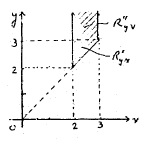
\includegraphics[width=0.7\textwidth]{images/b2p2-387-fig01.jpg}
    \end{minipage}\\
    
    Then 
    \begin{align*}
         I &= \int_{2}^{3} \quad \int_{x}^{\infty} \ \frac{1}{y^{2}} \ln \ \ln x \: dy \: dx \\ 
         &= \int_{2}^{3}  \ -\frac{1}{y} \ln \ \ln \ x\big|_{x}^{\infty} \: dx = \ \int_{2}^{3}  \ \frac{\ln \ln x}{x} \, dx \\
        &= \int_{2}^{3}  \ \ln \ \ln x \, d \, ln  x = \int_{u_1}^{u_2} \ln \,u \ du    
    \end{align*}
    
    
    
    
    
\end{document}